\documentclass[12pt]{article}
\usepackage[utf8]{inputenc}
\usepackage{amsmath, amssymb}
\usepackage{mathtools}
\usepackage{xcolor}
\usepackage{graphicx}
\usepackage[margin=1in]{geometry}
\usepackage{gensymb}
\usepackage{enumitem}
\usepackage{amsthm}
\usepackage{yfonts}


\usepackage{titlesec}

\definecolor{periwinkledark}{RGB}{102, 102, 128}
\newcommand{\rh}[1]{\textcolor{periwinkledark}{VP: #1 }}

\title{\bf The Continuum Hypothesis}

\titleformat{\chapter}
  {\normalfont\LARGE\bfseries}{\thechapter}{1em}{}
\titlespacing*{\chapter}{0pt}{3.5ex plus 1ex minus .2ex}{2.3ex plus .2ex}

\author{ Carl Tang, Xingkai Wang, Daniel Charbonneau, Mateo Muro, Vedant Puri
}
\date{24 April 2018}

\theoremstyle{definition}
\newtheorem{definition}{Definition}[section]
\newtheorem{theorem}{Theorem}[section]
\newtheorem{corollary}{Corollary}[theorem]
\newtheorem{lemma}{Lemma}[section]


\begin{document}
\maketitle

\tableofcontents

\newpage


\section{Comparing Cardinalities of Infinite Sets}
The Continuum Hypothesis (abbreviated CH) is a statement about the class of infinite cardinals. It was put forward in 1878 by Georg Cantor, the inventor of set theory. It is a statement on the nature of infinity in mathematics. The Continuum Hypothesis states that
\begin{center}
    \textit{
    There is no set whose cardinality is strictly between that of the integers and the real numbers.
    }
\end{center}

\noindent Let us begin with some definitions.
\begin{definition}
    The cardinality of some set $A$, denoted $|A|$, is a measure of the number of elements in a set. Set $A$ has cardinality $k$ $\iff\exists f:A\to \{1,2,..,k\}$ where $f$ is a bijection.
\end{definition}

We can compare the sizes of two sets by comparing their cardinal numbers. Two sets, $A$ and $B$, have the same cardinality, i.e. $|A|=|B|\iff f:A\to B,$ where $f$ is a bijection. We can define a relation $\leq$ on $C,$ the class of all cardinals, (we consider the class of all cardinals instead of the set of all cardinals to avoid Russel's paradox). We define the relation as follows:

\begin{definition}
    $(C,\leq)$ is a relation on $C.$ $\forall a,b\in C, a\leq b \iff\exists f:A\to B,$ where $f$ is an injection.
\end{definition}

$(C,\leq)$ is reflexive since $\text{id}:A\to A$ is a bijection. $(C,\leq)$ is antisymmetric since it can be proven that if $\exists f:A\to B,g:\B\to A$ where $f, g$ are injections, then there exists a bijection from $A$ to $B.$ It can also be proven that $(C,\leq)$ is transitive. Therefore $(C,\leq)$ is a partial order. Through Zorn's lemma, which is equivalent to the axiom of choice, one can prove that $(C,\leq)$ is a total order.

The total order on $C$ allows us to compare the sizes of any two sets. Specifically, for any two sets, $A, B$, either $|A|\leq |B|$ or $|B|\leq |A|$. If both statements are true, then $|A|=|B|$. The Continuum Hypothesis is concerned with the cardinalities of $\mathbb{N},$ the set of natural numbers, and $\mathbb{R},$ the set of real numbers. We denote $|
\mathbb{N}|$ as $\aleph_0$, pronounced 'aleph naught' after its symbol, the Hebrew letter Aleph.

In this section, we prove, first, that the cardinality of $\mathbb{N}$ is less than that of the real numbers through the famous diagonal argument put forward by Cantor. We further prove that the reals are equinumberous to the power set of natural numbers, i.e. $|\mathbb{R}|=2^{\aleph_0}$.

\begin{theorem}
    $\aleph_0 < |\mathbb{R}|$
\end{theorem}
\begin{proof}
    We first prove that $\aleph_0 \leq |\mathbb{R}|$ and then $\aleph_0 \neq |\mathbb{R}|$. Consider function $g:\mathbb{N}\to\mathbb{R}, g(k)=k$. It is trivial to check that $g$ is an injection. Hence $\aleph_0 \leq |\mathbb{R}|$.
    
    The second part is proved by contradiction. Consider, \textit{ad absurdum}, there exists a surjective function $f:\mathbb{N}\to[0,1]$. This means that all elements in $[0,1]\in\mathbb{R}$ can be enumerated as follows:
    \begin{align*}
        f(1)&=a_1=0.a_{11}a_{12}a_{13}a_{14}.. \\
        f(2)&=a_2=0.a_{21}a_{22}a_{23}a_{24}.. \\
        f(3)&=a_3=0.a_{31}a_{32}a_{33}a_{34}.. \\
        ... \\
        f(k)&=a_k=0.a_{k1}a_{k2}a_{k3}a_{k4}.. \\
    \end{align*}
    where each $a_i\in[0,1]$ is written in decimal expansion that does not end in repeating nines (since, for example $0.12\overline{99}=0.13$). Consider $b=0.b_1b_2b_3b_4...\in[0,1]$ defined such that $\forall i\in\mathbb{N},b_i\neq a_{ii}.$ Since $f:\mathbb{N}\to[0,1]$ is surjective, $\exists k\in\mathbb{N}, f(k)=a_k=b$. Since decimal expansions are unique (if we ignore infinitely repeated nines), $a_kk=b_k\bot$. Hence, there exists no surjective function from $\mathbb{N}$ to $[0,1]$.
    
    Therefore, $\aleph_0 < |\mathbb{R}|$.
\end{proof}

\begin{theorem}
    $|\mathbb{R}| = 2^{\aleph_0}$
\end{theorem}
\begin{proof}
    We first prove $|\mathbb{R}|\leq2^{\aleph_0}$ and then $2^{\aleph_0}\leq|\mathbb{R}|$. Every real number is composed of an integer component and an infinite decimal expansion. The decimal expansion can be put into one to one correspondence with $\mathbb{N}$. Hence, each real number has  $\aleph_0$ digits in its expansion.
    
    $$|\mathbb{R}|\leq \aleph_0\cdot10^{\aleph_0}\leq2^{\aleph_0} \cdot 2^{4\aleph_0}=2^{\aleph_0}$$
    
    To prove the second part, fix two digits (other than $0$ and $9$ to avoid ambiguity), say $2$ and $5$. The set of real numbers of the form $0.a_1a_2a_3a_4..$ where every $a_i$ is either $5$ or $7$ is in one-to-one correspondence with the set of all functions $f:\mathbb{N}^+\to \{2,5\}$. This gives us $2^{\aleph_0}$ distinct real numbers in the set, proving $2^{\aleph_0}\leq|\mathbb{R}|$. Therefore, $|\mathbb{R}| = 2^{\aleph_0}$.
\end{proof}

We denote the smallest cardinal greater than $\aleph_0$ as $\aleph_1$. The Continuum Hypothesis claims that $\mathbb{R}$ have the minimum possible cardinality greater than that of $\mathbb{N}$, i.e. $|\mathbb{R}|=\aleph_1$. The \textbf{Generalized Continuum Hypothesis} states that the cardinality of the power set of an infinite set is the smallest cardinality greater than that of the set. i.e. for any ordinal $\alpha,$ $\aleph_{\alpha+1} = 2^{\aleph_\alpha}$.


\section{Independence from Zermelo–Fraenkel Set Theory}
\subsection{Gödel's Proof of Consistency with ZFC}
Gödel proved that CH is consitent with the ZF set theory by comparing two different models of the ZF. The models he used are called the von Neumann Universe and the Constructible Universe. 
\begin{definition}
    \\Let $V_0=\emptyset$, for any ordinal $\beta$, $V_{\beta+1}=\wp(V_\beta)$, and for limit ordinal $\lambda$, $\bigcup\limits_{\beta<\lambda} V_\beta$. Then, we define $V:=\bigcup\limits_{\beta} V_\beta$ to be the \textbf{von Neumann Universe}. 
\end{definition}
Note that if we assume the axiom of regularity, then V is equivalent to the class of all sets.
\begin{definition}
    \\Gödel defined the following 10 operations, which we call \textbf{Gödel operations}: 
    \begin{enumerate}
        \item $G_1(X,Y)=\{X,Y\}$
        \item $G_2(X,Y)= X\times Y$
        \item $G_3(X,Y)=\{(x,y)|x\in X,y\in Y,x\in y\}$
        \item $G_4(X,Y)=X-Y$
        \item $G_5(X,Y)=X\cap Y$
        \item $G_6(X)=\cup X=\{x|\exists y\in X$ s.t $x\in y\}$
        \item $G_7(X)=dom(X)=\{x|\exists y $ s.t $[x,y]\in X\}$
        \item $G_8(X)=\{(x,y)|(y,x)\in X\}$
        \item $G_9(X)=\{(x,y,z) | (x,z,y)\in X\}$
        \item $G_{10}(X)=\{(x,y,z)|(y,z,x)\in X\}$
    \end{enumerate}
\end{definition}
\begin{definition}
    \\For any set $X$, we define the \textbf{Gödel closure} of $X$, denoted $cl(X)$, to be the smallest set containing $X$ s.t it's closed under Gödel operations. \\Equivalently, $cl(X)=\bigcup\limits_{i\in \mathbb{N}} G^i(X)$ where $G(X)=\{G_i(x,y)|x,y\in X, 1\leq i \leq 10\}$
\end{definition}
\begin{definition}
   \\We define the \textbf{logically definable subsets} of $X$:\\ $Def(X):= cl(X\cup \{X\}) \cap \wp (X)$
\end{definition}
\begin{definition}
    \\Let $L_0=\emptyset$, for any ordinal $\alpha$, $L_{\alpha +1}=Def(L_\alpha)$, and for any limit ordinal $\lambda$, $L_\lambda=\bigcup\limits_{\alpha < \lambda} L_\apha$. Then, we define $L:=\bigcup\limits_{\alpha} L_\alpha$ to be the \textbf{Constructible Universe}. We call a set $S$ constructible if and only if for some ordianl $\alpha$, $S\in L_\alpha$
\end{definition}
Both V and L are models of the ZF theory, i.e. $V\models ZF$ and $L\models ZF$. Further, both are towers of transitive sets (they are also transitive classes), meaning that $(\forall x\in V_\beta$ or $L_\alpha$, $y\in x \implies y \in V_\beta$ or $L_\alpha)$, and that $\forall i\leq j$, $V_i\in V_j, L_i\in L_j$.  
\begin{definition}
    Gödel introduced the \textbf{Axiom of Constructibility}: $V=L$, i.e. all sets (assuming the axiom of regularity) are constructible.
\end{definition}
Now, we want to prove that $L$ actually models the axiom of constructiblity. 
\begin{definition}
    Let $M$ be a transitive class, and let $\psi(x_1,...,x_n)$ be a formula, we say that $\psi$ is \textbf{absolute} for $M$ if that $M\models \psi(x_1,...,x_n) \iff \forall x_1,...,x_n\in M$, $\psi(x_1,...,x_n)$ holds.
\end{definition}
\begin{lemma}
If $\psi$ is restricted, then $\psi$ is absolute in transitive class $M$. \\(restricted means that $\psi$ is of the form ($\forall u\in X$ or $\exists u\in X$))
\end{lemma}
\begin{definition}
    Let $\phi$ be the following expression: 
    \begin{itemize}
        \item $\forall x,y$ and $1\leq i \leq 10$, $\exists z$ s.t $z=G_i(x,y)$
        \item $\forall x$, $\existsy=cl(x)$
        \item $\forall$ ordinals $\alpha$, $\exists$ a family $\{L_\beta|\beta < \alpha\}$ s.t $L_0=\emptyset$, $L_{\beta+1}=Def(L_\beta)$, for limit ordinal $\lambda$, $L_\lambda=\bigcup\limits_{\beta<\lambda}L_\beta$
    \end{itemize}
    We call a set (class) $M$ \textbf{adequate} if $M\models \phi$.
\end{definition}
\begin{lemma}
If $M$ is transitive and adequate, then $\forall$ ordinal $\alpha \in M$, $(x\in L_\alpha)$ is absolute. 
\end{lemma}
\begin{definition}
    A set $M$ is called extensional if for any distinct $x,y\in M$, $\exists z\in M$, $z\in x$ or $z\in y$, but $z\notin x\cap y$.
\end{definition}
\begin{lemma}
\textbf{(Reflection Principle)} Let $M_0$ be a countable set and let $\psi(v_1,...,v_n)$ be a formula. Suppose $\psi(x_1,...,x_n)$ is true for some $x_1,...,x_n\in M_0$. Then, $\exists$ a countable set $M$ s.t $M_0\subseteq M$, $M$ is extensional, and $M\models \psi(x_1,...,x_n)$
\end{lemma}
\begin{theorem}
Let $M$ be an extensional set. Then $\exists$ a transitive set $N$ which is isomorphic to $M$, i.e. $\exists$ bijection $f:M\to N$ s.t $x\in y \iff f(x) \in f(y)$. For any formula $\psi (v_1,...,v_n)$ and any $x_1,...,x_n \in M$, we have $M \models \psi(x_1,...,x_n) \iff N \models \psi (f(x_1),...,f(x_n))$
\end{theorem}
\begin{lemma} 
\\\
\begin{enumerate}[label=(\roman*)]
\item The function $\alpha \mapsto L_\alpha$ is absolute for transitive models of ZF 
\item If $M$ is a transitive model of ZF containing all ordinals, then ``$x$ is constructible" is absolute for $M$, and in fact $L^M = L$ ($L^M$ is the corresponding class in M of L) 
\end{enumerate}
\end{lemma}
Consequently, $L^M=L \implies L\subseteq M$ for any transitive model of ZF containing all odrinals. If $x\in L$, then 
\begin{center}
    $L\models x$ is constructible 
\end{center}
and thus $L$ satisfies the axiom of constructibility. Now that we know the axiom of constructibility is consistent with $L$, where $L$ models ZF, it suffices to show that the axiom of constructibility implies CH. 
\begin{theorem}\label{thm:main}
$V=L \implies 2^{\aleph_\alpha}=\aleph_{\alpha+1}$
\end{theorem}
The key element of the proof is the following lemma: 
\begin{lemma}\label{lmm:main}
Assume $V=L$. If $X\subseteq \omega_\apha$, then $\exists \gamma < \omega_{\alpha +1}$ s.t $X\in L_\gamma$
\end{lemma}
\begin{proof}[Proof of theorem \ref{thm:main}]\footnote{This particular proof is from page 110, Jech, Thomas J. Set Theory. Academic Press, 1978. ISBN 9780080873954. This whole section follows loosely the second chapter of this book.}
Assume that $V=L$. By Lemma 2.5, every subset of $\omega_\alpha$ is constructible before the stage $\omega_{\alpha+1}$, i.e.,  $\wp(\omega_\alpha)\subseteq L_{\omega_{\alpha+1}}$. it is easy to show by induction that for every $\gamma \geq \omega$, $|L_\gamma|=|\gamma|$, and so $|L_{\omega_{\alpha+1}}|=\aleph_{\alpha+1}$. Therefore, $|\wp(\omega_\alpha)|=\aleph_{\alpha+1}$.
\end{proof}
\begin{proof}[Proof of lemma \ref{lmm:main}]
The proof of the lemma makes use of most of the previous lemma and definitions, but I won't put it on here since it is fairly long. It is shown on page 112 of Professor Jech's \textit{Set Theory}. 
\end{proof}
\subsection{Cohen's Proof of Independence from ZFC}
In this section, we illustrate the main techniques developed by Cohen in his proof of independence of CH from ZFC. Cohen used what is now called forcing in order to start with a universe U that abides by ZFC, and then expand it into a new universe U' where a new subset of cardinal numbers which did not exist in U, thus violating the Continuum Hypothesis. Instead of Cohen's proof, here is another proof using forcing to show how to collapse cardinals.

Start with set U which follows ZFC. Let k and w be uncountable and countable cardinals in U, respectively. Thus there is no bijection mapping k to w. Define set A as the set of all partial functions from k to w, and define $\leq$ as for any p,q in A, p $\leq$ q if and only if p is an extension of q as a function. Thus (A, $\leq$) is a partially ordered set. Consider a generic ideal G of A (the trait most important to this proof is that for any subset D of A is dense, the intersection of D and G is not empty. Here, dense means for any p in A and subset D of U, there exists q in D such that q $\leq$ p).

Define f as the union of all p such that p is an element of G. For each n in w, define N as the set of all p in A such that n is in the domain of p). N is dense, as for any p, if n does not exist in the domain of p, it is possible to adjoin a value for n such that it exists in N, this is by definition in N. Because G is a generic ideal, without loss of generality we can assume there exists a p in the intersection of G and N, and p is an element of f, so n exists in the domain of f. This proves f is injective, as the intersection of G and N is not empty by definition for all n.

For each a in k, define K as the set of all p in A such that a is in the range of p. By the same argument as above, K is dense so there exists a p in the intersection of G and K, p is an element of f, and a is in the range of f, the intersection of G and K is not empty for any k, so f is surjective, Thus f is bijective, so k is by definition countable in the union of U and G, something that was not the case in just U.

Cohen was able to use a similar method to prove that it is possible to construct a U' in which there exists subsets of cardinals that did not exist in U. Therefore, in ZFC, it is impossible to prove the Continuum Hypothesis. So it is inconsistent, and together, with Gödel's work, this proves that the Continuum Hypothesis is independent of the axioms of ZFC.


\section{Some Interesting Countable Sets}
Let us begin with some definitions.
\begin{itemize}
    \item $\omega$ denotes the set of natural numbers, $\omega^\omega$ denotes the set of infinite subsets of natural numbers, and $^\omega\omega$ denotes the set of all functions from natural numbers to natural numbers.
    \item Two countable, infinite sets are \textit{almost disjoint} provided their intersection is finite. A family of pairwise almost disjoint subsets of a set X is \textit{maximal} provided it is not properly contained in another pairwise disjoint almost disjoint family of subsets of X.
    \item For $A, B$ in $\omega^\omega$, we say $A$ is \textit{almost included} in $B$ (denoted $A\subseteq^*B$) provided $A-B$ is finite.
    \item For a family $F\subseteq\omega^\omega$, we say that $F$ has the \textit{strong finite intersection property} provided every finite subfamily has an infinite intersection, and an infinite set $A$ is called a \textit{pseudointersection} of $F$ provided $A\subseteq^*f$ for all $f\subseteq F$.
    \item A family $T\subseteq\omega^\omega$ is a $tower$ provided that it is well-ordered by $\subseteq^*$.
    \item A family $U\subseteq\omega^\omega$ \textit{generates an ultrafilter} provieded every finite intersection of elements of $U$ contains an elements of $U$, and for every $A\in\omega^\omega$ either there exists $B\in U$ such that $U\subseteqA$, or there exists $B\in U$ such that $U\subseteq\omega-A$. An ultrafilter base $U$ is called free provided \cap U=\emptyset.
    \item A family $I\subseteq\omega^\omega$ is an \textit{independent family} provided for every finite subfamilies $A, B\in I$, if $A\neq\emptyset$ and $A\cap B=\emptyset$ then $\cap A-\cup B\neq\emptyset$.
    \item A family $S\subseteq\omega^\omega$ is a \textit{splitting family} provided for every $A, B\in\omega^\omega$, there exists $B\in S$ such that $|A\cap S|=|A-S|=\omega$.
    \item Define the \textit{mod finite order} $\leq^*$ (a reflexive transitive order) on the set $^\omega\omega$ as follows: for $f,g\in ^\omega\omega$ we say $f\leq^*g$ provided there exists $N\in \omega$ such that for all $n\geq N, f(n)\leq g(n)$.
    \item A set $X\subseteq ^\omega\omega$ is $dominating$ (in the mod finite order) provided for every $f\in ^\omega\omega$ there exists $g\in X$ such that $f\leq^* g$, and $X$ is $bounded$ (in the mod finite order) if there exists $g\in ^\omega\omega$ for all $f\in X$
    \item \textswab{a}=min\{$|A|:A\subseteq\omega^\omega$ is an infinite, maximal almost disjoint family in $\omega\}$
    \item \textswab{b}=min\{$|B|:B\subseteq^\omega\omega$ is unbounded in the mod finite order\}
    \item \textswab{d}=min\{$|D|:D\subseteq^\omega\omega$ is dominating in the mod finite order\}
    \item \textbf{s}=min\{$|S|:S\subseteq\omega^\omega$ is a splitting family\}
    \item \textswab{p}=min\{$|P|:P\subseteq\omega^\omega$ has the strong finite intersection property but no pseudointersection\}
    \item \textswab{t}=min\{$|T|:T\subseteq\omega^\omega$ is a tower on $\omega$\}
    \item \textswab{i}=min\{$|I|:I\subseteq\omega^\omega$ is a maximal independent family on $\omega$\}
    \item \textswab{u}=min\{$|U|:U\subseteq\omega^\omega$ generates an ultrafilter on $\omega$\}
    \item \textswab{c} is the cardinality of the set of real numbers, and $\aleph_1$ denotes the cardinality of the smallest uncountable cardinal
\end{itemize}

\begin{center}
    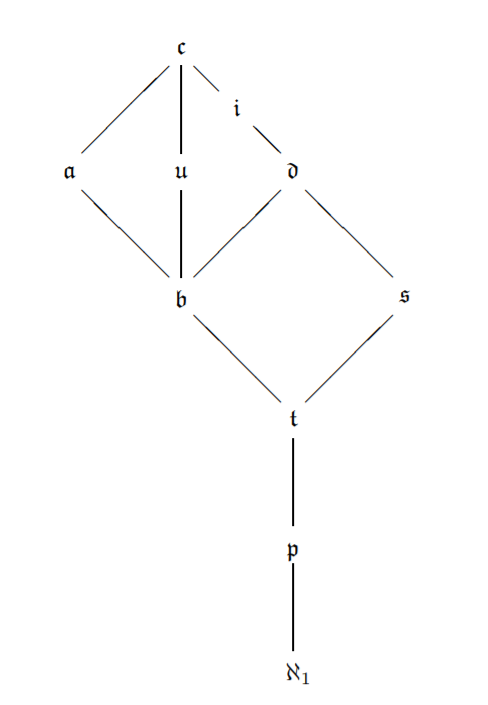
\includegraphics[width=10cm, height=15cm]{diagram}
\end{center}
This graph shows the partial order relationships between these uncountable cardinal numbers. There have been efforts to make some of these inequalities strict, but to no avail. The mathematics community believes this problem to be either independent of ZFC not provable. The most interesting problem is determining if \textswab{p}$<$\textswab{t}, as it would give us a model into an uncharted territory where \textswab{c}$\geq\aleph_3$. However, in 2015, Mallaris and Shelah proved that \textswab{p}=\textswab{t}, a surprising result. Following is the brief idea of the proof that Mallaris and Shelah gave.
\begin{theorem}
    \textswab{p}=\textswab{t}
\end{theorem}
\begin{proof}
    Let $s$ be a cofinality spectrum problem, then $C(s,t\_s)=\emptyset$. This is actually the central theorem in their paper, and it will later be used to prove \textswab{p}=\textswab{t}. They defined some special forcing sets and a transitive model of ZFC. They showed that they can extend this model of ZFC to a new model with one set they defined, and showed that these sets can together form a cofinality spectrum problem related to \textswab{p} and \textswab{t}. Then, \textswab{p}=\textswab{t}
\end{proof}

This proof shows that when assuming \textswab{p} < \textswab{t}, one can arrive at a contradiction with the central theorem of this paper, and $\textswab{p}\leq\textswab{t}$ is known from the diagram. Therefore, \textswab{p}=\textswab{t}. This is a very interesting result in the development of set theory. Hopefully, someone can extend on this paper and prove more intriguing facts about these cardinals or many other cardinals.



\section{Formalism in Mathematics}
The philosophy of mathematics has been turned on its head since Cantor's set theory was introduced. Similarly, the continuum hypothesis has led to some developments, as well as new debates. We start with Hilbert's Program, which had two goals:
\begin{enumerate}
    \item Show that all mathematical truths follow from a (finite) set of axioms
    \item Show that such an axiomatic system is consistent
\end{enumerate}

A lofty goal it may seem at first, Hilbert believed that mathematics would prevail. ZFC is now considered fundamental mathematics, and you may think that something like that would prove to be the foundation of mathematics that Hilbert and other formalists were looking for. Alas, Gödel proved Hilbert's program to be a failure. We first define some notions of axioms.

\begin{definition}
    An axiom $\phi$ is independent of other another set of axioms $F$ if $F$ cannot derive $\phi$ or $\neg\phi$.
\end{definition}

\begin{definition}
    A set of axioms $F$ is consistent if it is never possible to derive a contradiction $F$.
\end{definition}

\begin{definition}
    A set of axioms $F$ is complete if for every statement $\phi$, F can either derive $\phi$ or $\neg\phi$.    
\end{definition}

We now state Gödel's two Incompleteness theorems.

\begin{theorem}
    Assume $F$ is a consistent (finite) set of axioms that can model arithmetic. Then there exists statements of arithmetic that $F$ can neither prove nor disprove, i.e. $F$ is incomplete.
\end{theorem}

\begin{theorem}
    Assume $F$ is a consistent (finite) set of axioms that can model arithmetic. Then $F$ can not prove its own consistency.
\end{theorem}


This shook the foundation of mathematics for most people and gave plenty of problems for Hilbert's program. Some will say that there just needs to be a readjusting of our axiomatic approach, but axiomatic set theory as we know it now fails to describe all of mathematics, and that is why we have undecidable propositions such as the continuum hypothesis.

There are two main intelligible responses to undecidable propositions such as CH. TThe first is the pluralist school, which Cohen and many modern mathematicians subscribe to. This view says the independence result shows that because both CH and $\neg$ CH are possible, that neither is more "correct" than the other. The question "Is the continuum hypothesis true?" is nonsensical to pluralists without being given a model that decides the proposition, almost like asking "Is a number even?" without specifyng which number one is speaking about.

To contrast that is the nonpluralist, such as Gödel. Gödel seemed convinced that there is a fact of the matter in mathematics. This is because Gödel still believed that some of the unprovable statements in his First Incompleteness Theorem were still true. After all, the statement was "This sentence is not provable." You also add the fact that in his proof outlined above, he uses the axiom of constructability to derive the genrealized CH. He believed that we simply needed to add more axioms that mathematicians could agree upon that would decide CH or $\neg$ CH. This would be consistent with out previous notion of mathematics being complete, so it is ironic tha the man who proved math to be incomplete to be such a strong proponent of nonpluralism.



\newpage
\begin{thebibliography}{9}
\bibitem{1}
    Kaplansky, I. \textit{Set Theory and Metric Spaces,} Boston: Allyn and Bacon, Inc., 1977.
\bibitem{4}
    Mill, J. V. (1990). Open problems in topology. Retrieved April 21, 2018, from https://pdfs.semanticscholar.org/9065/61a1e45b49a2ab816e088ffd33279c05a3ba.pdf
\bibitem{3}
    Malliaris, M., & Shelah, S. (2015). Cofinality spectrum theorems in model theory, set theory, and general topology. Journal of the American Mathematical Society, 29(1), 237-297. doi:10.1090/jams830

\bibitem{2}
    William (https://math.stackexchange.com/users/13579/william), What are some simple example of "forcing" in set theory?, (version: 2015-06-04): https://math.stackexchange.com/q/1311794



\end{thebibliography}



\end{document}